\begin{minipage}[b]{190mm}
\fcolorbox{black}{white}{
\begin{minipage}[b]{0.35\linewidth}
\Huge \textbf{UNF NEWS} \\
\Large -- I før-fremtid har katte det godt!
\end{minipage}
\begin{minipage}[b]{0.4\linewidth}
\Large Søndag 14.07.2012 \\
\normalsize Redigeret i \LaTeX\ af \\ SOM, MGS, WIL

\end{minipage}
}
\end{minipage}

\begin{minipage}[b]{0.95\linewidth}
\begin{minipage}[t]{0.47\textwidth}
\vspace{1mm}
\section*{Nijas dagbog}
Jeg kommer til at vide, at denne dag, ikke var den bedste i mit liv. Jeg vil være blevet vækket af marcherende militærstøvler i de nordnorske bjerge, kort efter blive bortført sammen med storesøster og min tynde tvilling. Jeg vil være blevet bragt til et osende fly, og fløjet sydpå til skrigenes by og videre til stedet ingenører sidder i rundkreds og stønner. Op på en lastvogn af tysk mærke vil vi være blevet smidt og sydpå fragtet i høj fart. Men i det mindtjydske vil vores familiebånd hendfalde under fysikernes strålekanon, og mens hydroxiden, og dermed min arvepart til sæteren, forsvandt mod undergangen i Preussernes varetægt, vil jeg, ensom og alene, sidde på en jysk bakketop


\end{minipage}%
\hfill\begin{minipage}[t]{0.47\textwidth}
\vspace{1mm}
\section*{Vejrudsigt}
\textbf{IMF, AU (fra DMI)}: Skyer, men med synlig sol. Op til 18 grader om dagen og ned til 12 grader om natten, ingen regn.

\textbf{IMF, AU år 2003}: Tør med dagstemperaturer op til 26 grader og nattemperaturer ned til 8 grader, 14 timers sol og næsten skyfri himmel.

\section*{Fakt om Jylland}
Jylland er ikke verdens største ø

\section*{Dagens sandsynlighed}
Sandsynligheden for at din hjerne indeholder et atom der indgik i en dinosaur er cirka $1$.

\section*{Find en Fynbo}
Rygtet siger at der har sneget sig en Fynbo ind i dette ærkejydske blad. Dette kan selvfølgelig ikke accepteres, og halvsvenskeren må derfor opspores og udraderes.

\section*{Dagens datalog}
Hvis du møder en datalog, prik ham og påpeg at der er en syntaxfejl i whitespackoden i hans blanke blik.

\section*{Ordforklaring: Whitespace}
\vspace{4cm}
%\vspace{-1.2cm}
%\begin{center}
%$\quad$\hspace{4cm}
%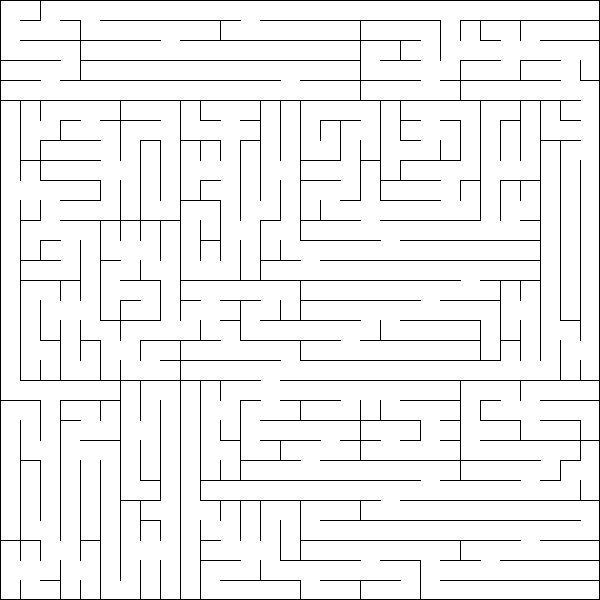
\includegraphics[width=0.8\linewidth]{maze.jpg}
%\end{center}
%\vspace{-5.7cm}
\end{minipage}

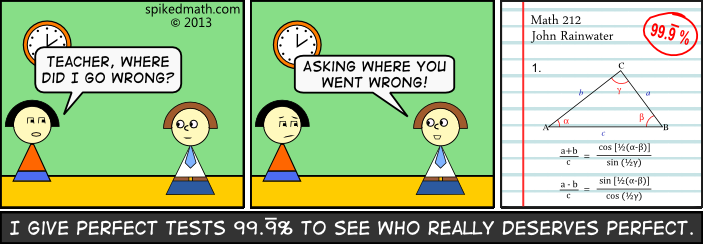
\includegraphics[width=0.9\textwidth]{547-the-perfect-score.png}
\begin{center}
\tiny Mike, http://http://spikedmath.com/547.html, CC-BY-NC-2.5
\end{center}
\end{minipage}

